\documentclass{article}
\usepackage{graphicx, amsmath, amssymb, mathtools, fancyhdr}

\graphicspath{{Images/}}

\setlength{\oddsidemargin}{0in}
\setlength{\textwidth}{6.5in}
\setlength{\topmargin}{-.55in}
\setlength{\textheight}{9in}
\pagestyle{fancy}

\fancyfoot{}
\fancyhead[R]{\thepage}
\fancyhead[L]{MATH 6440}

\begin{document}

\begin{center}
    {\huge $\text{sinc}^2$ Integral}
    \vspace{0.5cm}

    {\large Michael Nameika}
\end{center}
Show 
\[\int_{0}^{\infty}\frac{\sin^2(x)}{x^2}dx = \frac{\pi}{2}\]
\textit{Proof:} We first show that the integral converges. Note that $\frac{\sin^2(x)}{x^2}$ has a removable singularity at $x = 0$ since ${\displaystyle \lim_{x \to 0}\frac{\sin(x)}{x} = 1}$. Thus, $\frac{\sin^2(x)}{x^2}$ is integrable near $x = 0$. Further notice, for $R > 0$
\begin{align*}
    \left|\int_R^{\infty}\frac{\sin^2(x)}{x^2}\right| &\leq \int_R^{\infty}\left|\frac{\sin^2(x)}{x^2}\right|dx\\
    &\leq  \int_R^{\infty}\frac{1}{x^2}dx\\
    &= \frac{1}{R} < \infty.
\end{align*}
Thus, the integral converges. Now, we approach this in two ways.
\begin{itemize}
    \item[(a)] \textbf{Approach 1.} Consider the function $f(z) = \frac{1 - e^{2iz}}{z^2}$ over the indented semicircle contour. 

    \begin{center}
        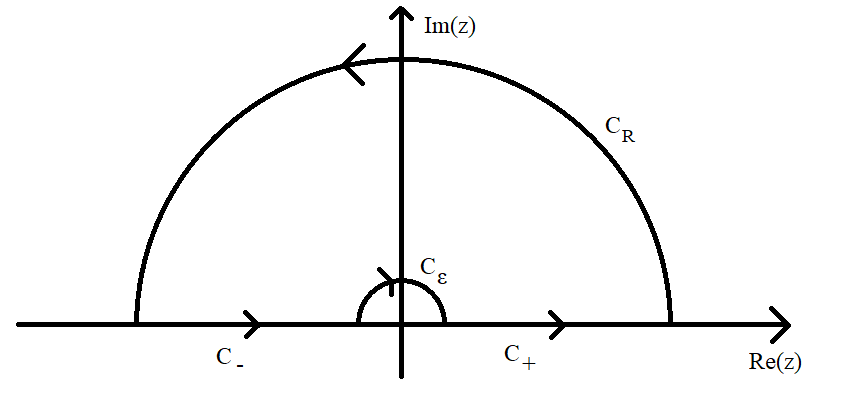
\includegraphics[scale = 0.4]{contour1.PNG}
    \end{center}
    By Cauchy's theorem, since $f(z)$ is analytic in and on $C$,
    \[\oint_Cf(z) = 0.\]
    
    For $C_R$, parameterize $z = Re^{i\theta}$, $dz = Rie^{i\theta}d\theta$. Then 
    \begin{align*}
        \int_{C_R}\frac{e^{2iz} - 1}{z^2}dz &= \int_0^{\pi}\frac{e^{2iRe^{i\theta}} - 1}{R^2e^{2i\theta}}Rie^{i\theta}d\theta\\
        &=\frac{i}{R}\int_0^{\pi}\frac{e^{2iR\cos(\theta)}e^{-2R\sin(\theta)}-1}{e^{i\theta}}d\theta\\
        \implies \left|\int_{C_R}f\right| &\leq \frac{1}{R}\int_0^{\pi}\left|\frac{e^{2iR\cos(\theta)}e^{-R\sin(\theta)} - 1}{e^{i\theta}}\right|d\theta\\
        &\leq \frac{1}{R}\int_0^{\pi}\left(e^{-2R\sin(\theta)} + 1\right)d\theta\\
        &= \frac{\pi}{R} + \frac{1}{R}\int_0^{\pi}e^{-2R\sin(\theta)}d\theta\\
        &= \frac{\pi}{R} + \frac{2}{R}\int_0^{\pi/2}e^{-2R\sin(\theta)}d\theta.
    \end{align*}
    Note that for $\theta \in [0,\pi/2]$, $\sin(\theta) \geq \frac{2}{\pi}\theta \implies -2R\sin(\theta) \leq -\frac{4}{\pi}R\theta$ hence
    \begin{align*}
        \left|\int_{C_R}f\right| &\leq \frac{\pi}{R} + \frac{2}{R}\int_0^{\pi}e^{-\frac{4}{\pi}R\theta}d\theta\\
        &= \frac{\pi}{R} + \frac{2}{R}\left[-\frac{\pi}{4R}e^{-\frac{4}{\pi}R\theta}\right]\bigg|_0^{\pi/2}\\
        &= \frac{\pi}{R} - \frac{\pi}{2R^2}e^{-2R} + \frac{\pi}{4R^2}\\
        &\to 0 \hspace{0.5cm} \text{as} \hspace{0.5cm} R \to \infty.
    \end{align*}
    Now, on $C_{\varepsilon}$, Taylor expanding $e^{2iz}$ gives 
    \[e^{2iz} = 1 + 2iz - 2z^2 - \frac{4i}{3}z^3 + \cdots\]
    so that the integral becomes
    \begin{align*}
        \int_{C_{\varepsilon}}\frac{e^{2iz} - 1}{z^2}dz &= \int_{C_R}\frac{1 + 2iz - 2z^2 - \tfrac{4i}{3}z^3 + \cdots - 1}{z^2} dz \\
        &= \int_{C_{\varepsilon}}\frac{1}{z}\left(2i - 2z - \frac{4}{3}z^2 + \cdots\right)dz
    \end{align*}
    now parameterize $z = \varepsilon e^{i\theta}$, $dz = \varepsilon ie^{i\theta}d\theta$. Then the above integral becomes
    \begin{align*}
        \int_{\pi}^0 \frac{1}{\varepsilon e^{i\theta}}\left(2i - 2\varepsilon e^{i \theta} + \cdots\right)\varepsilon i e^{i\theta}d\theta &= i\int_{\pi}^0\left(2i - 2\varepsilon e^{i\theta} + \cdots\right)d\theta\\
        &= 2\pi + 4\varepsilon + \mathcal{O}(\varepsilon^2)\\
        &= 2\pi \hspace{0.5cm} \text{as} \hspace{0.5cm} \varepsilon \to 0.
    \end{align*}
    Further, as $\varepsilon \to 0$ and $R \to \infty$, 
    \begin{align*}
        \int_{C_-}f + \int_{C_+}f &\to \int_{-\infty}^{\infty} \frac{e^{2ix} - 1}{x^2} dx\\
        &= \int_{-\infty}^{\infty}\frac{\cos(2x) - 1}{x^2}dx + i\int_{-\infty}^{\infty}\frac{\sin(2x)}{x^2}dx\\
        &= -2\int_{-\infty}^{\infty}\frac{\sin^2(x)}{x^2}dx + i\int_{-\infty}^{\infty}\frac{\sin(2x)}{x^2}dx
    \end{align*}
    and note that the imaginary part of the above integral converges in the principle value sense. Putting it together, we have
    \begin{align*}
        -2\int_{-\infty}^{\infty}\frac{\sin^2(x)}{x^2}dx + i\int_{-\infty}^{\infty}\frac{\sin(2x)}{x^2}dx + 2\pi &= 0\\
        \implies \int_{-\infty}^{\infty}\frac{\sin^2(x)}{x^2}dx &= \pi\\
    \end{align*}
    and since $\frac{\sin^2(x)}{x^2}$ has even parity and ${\displaystyle \int_0^{\infty} \frac{\sin^2(x)}{x^2}dx }$ converges, we have
    \[\int_0^{\infty}\frac{\sin^2(x)}{x^2}dx = \frac{\pi}{2}\]
    as desired.

    \item[(b)] \textbf{Approach 2.} Consider the function $f(z) = \frac{e^{2iz} - 1 - 2iz}{z^2}$. Note that $f$ has a removable singularity at $z = 0$. By L'Hopital's rule, we have
    \begin{align*}
        \lim_{z \to 0}\frac{e^{2iz} - 1 - 2iz}{z^2} &=\lim_{z \to 0} \frac{2ie^{iz} - 2i}{2z}\\
        &= \lim_{z\to 0} \frac{-4e^{iz}}{2}\\
        &= -2
    \end{align*}
    Define the auxillary function
    \[\hat{f}(z) = \begin{cases}
        f(z) & z \neq 0\\
        -2 & z = 0.
    \end{cases}\]
    We then integrate $\hat{f}(z)$ over the contour
    \begin{center}
        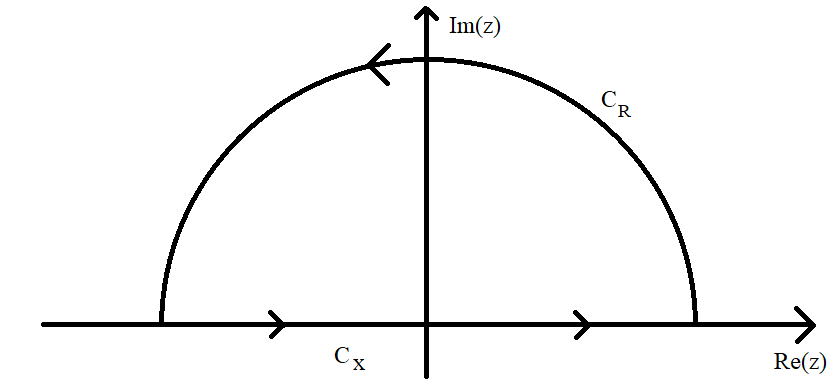
\includegraphics[scale = 0.4]{contour2.PNG}
    \end{center}
    By Cauchy's theorem, we have
    \[\oint_{C}\hat{f} = 0.\]
    On $C_R$, parameterize $z = Re^{i\theta}$, $dz = Rie^{i\theta}d\theta$. Then 
    \begin{align*}
        \int_{C_R} \hat{f}(z)dz &= \int_0^{\pi}\frac{e^{2iRe^{i\theta}} - 1 - 2iRe^{i\theta}}{R^2e^{2i\theta}}Rie^{i\theta}d\theta\\
        &= i\int_0^{\pi} \frac{e^{2iRe^{i\theta}}}{Re^{i\theta}}d\theta - i\int_0^{\pi}\frac{1}{Re^{i\theta}}d\theta + 2\pi\\
        &= i\int_0^{\pi}\frac{e^{2iRe^{i\theta}}}{Re^{i\theta}}d\theta - \frac{2}{R} + 2\pi.
    \end{align*}
    Now notice 
    \begin{align*}
        \left|i\int_0^{\pi}\frac{e^{2iRe^{i\theta}}}{Re^{i\theta}}d\theta\right| &\leq \frac{1}{R}\int_0^{\pi} \left|e^{2iR\cos(\theta) - 2R\sin(\theta)}\right|d\theta\\
        &= \frac{1}{R}\int_0^{\pi} e^{-2R\sin(\theta)}d\theta\\
        &= \frac{1}{R}\int_0^{\pi/2}e^{-2R\sin(\theta)}d\theta
    \end{align*}
    And notice that for $0 \leq \theta \leq \frac{\pi}{2}$, $\sin(\theta) \geq \frac{2}{\pi}\theta \implies -2R\sin(\theta) \leq -\frac{4R}{\pi}\theta$ hence
    \begin{align*}
        \frac{1}{R}\int_0^{\pi/2}e^{-2R\sin(\theta)}d\theta &\leq \frac{1}{R}\int_0^{\pi/2} e^{-\frac{4}{\pi}R\theta}d\theta\\
        &= \frac{1}{R}\left[-\frac{\pi}{4R}e^{-\frac{4}{\pi}R\theta}\right]\bigg|_0^{\pi/2}\\
        &= \frac{1}{R}\left[\frac{\pi}{4R} - \frac{\pi}{4R} e^{-2}\right]\\
        &\to 0 \hspace{0.5cm} \text{as} \hspace{0.5cm} R \to \infty.
    \end{align*}
    Thus, as $R \to \infty$, 
    \begin{align*}
        \int_{C_R} \hat{f} &\to 2\pi.
    \end{align*}
    Further, as $R \to \infty$,
    \begin{align*}
        \int_{C_x}\hat{f} &\to \int_{-\infty}^{\infty} \frac{e^{2ix} - 1 - 2ix}{x^2}dx\\
        &= \int_{-\infty}^{\infty} \frac{\cos(2x) + i\sin(2x) - 1 - 2ix}{x^2}dx\\
        &= \int_{-\infty}^{\infty}\frac{\cos(2x) - 1}{x^2}dx + i\int_{-\infty}^{\infty} \frac{\sin(2x) - 2x}{x^2}dx\\
        \implies \text{Re}\left(\int_{C_x}\hat{f}\right) &= -2\int_{-\infty}^{\infty}\frac{\sin^2(x)}{x^2}dx
    \end{align*}
    Now,
    \[\oint_{C}\hat{f} = \int_{C_x}\hat{f} + \int_{C_R}\hat{f} = 0\]
    \begin{align*}
        \implies -2\int_{-\infty}^{\infty}\frac{\sin^2(x)}{x^2}dx + i\int_{-\infty}^{\infty}\frac{\sin(2x) - 2x}{x^2}dx + 2\pi &= 0\\
        \implies \int_{-\infty}^{\infty}\frac{\sin^2(x)}{x^2}dx &= \pi\\
        \implies 2\int_0^{\infty}\frac{\sin^2(x)}{x^2}dx &= \pi\\
        \implies \int_0^{\infty} \frac{\sin^2(x)}{x^2}dx &= \frac{\pi}{2}
    \end{align*}
    As desired.

\end{itemize}

\end{document}
